\documentclass[10pt,xcolor=x11names,compress,aspectratio=169]{beamer}

%% =========================================================
%% Theme
%% =========================================================

\usetheme{Madrid}
\definecolor{mainblue}{RGB}{18,35,90}
\usecolortheme[named=mainblue]{structure}
\setbeamertemplate{footline}{%
  \begin{beamercolorbox}[wd=\paperwidth,ht=2.5ex,dp=1.5ex,center]{}%
    \usebeamerfont{footline}\color{mainblue}\insertframenumber
  \end{beamercolorbox}}
\setbeamertemplate{frametitle continuation}{}
\beamertemplatenavigationsymbolsempty
\setbeamerfont{title}{size=\Large}
\setbeamerfont{frametitle}{size=\large}
\setbeamertemplate{headline}{}
\setbeamertemplate{navigation symbols}{}

%% =========================================================
%% Packages
%% =========================================================

\usepackage{amsmath,amssymb,bm}
\usepackage{physics}
\usepackage{graphicx}
\usepackage{booktabs}
\usepackage{array}
\usepackage{multirow}
\usepackage{algpseudocode}
\algrenewcommand\algorithmicrequire{\textbf{Input:}}
\usepackage{tikz}
\usetikzlibrary{positioning,arrows.meta}
\usepackage{tcolorbox}
\tcbuselibrary{skins,breakable}
\usefonttheme{serif}

\graphicspath{{figures/}{./}}

%% =========================================================
%% Box Style
%% =========================================================

\tcbset{
  mybox/.style={
    enhanced, colback=white, colframe=mainblue,
    boxrule=0.6pt, arc=2pt,
    left=3pt, right=3pt, top=3pt, bottom=3pt
  }
}

%% =========================================================
%% Metadata
%% =========================================================

\title{%
  \parbox{0.78\linewidth}{\centering
    Rydberg Atomic Receivers\\
    for Future Wireless Communications}}
\author{P SRIHARI\\25SP06015}
\institute{M.Tech \\ Signal Processing \& Communications\\
  Indian Institute of Technology Bhubaneswar}

%% =========================================================
\begin{document}
%% =========================================================

%% ---- 1. Title (unchanged) --------------------------------
\begin{frame}[plain]
\begin{tikzpicture}[remember picture, overlay]

  \draw[mainblue, line width=1.2pt]
    ([yshift=-1.55cm]current page.north west) --
    ([yshift=-1.55cm]current page.north east);

  \node[anchor=north west, inner sep=0pt, text width=7cm, align=left]
    at ([xshift=12pt, yshift=-8pt]current page.north west)
    {\color{mainblue}\scriptsize
      \textbf{Indian Institute of Technology Bhubaneswar}\\[1pt]
      \textit{School of Electrical and Computer Science}};

  \node[anchor=north east, inner sep=0pt]
    at ([xshift=-10pt, yshift=-4pt]current page.north east)
    {\includegraphics[height=1.45cm]{IITBBS_Logo.png}};

  \node[anchor=center]
    at (current page.center)
    {\parbox{0.80\linewidth}{\centering
      {\color{mainblue}\LARGE\textbf{Rydberg Atomic Receivers\\[4pt]
      for Future Wireless Communications}}\\[10pt]
      {\normalsize\textbf{P SRIHARI}}\\[2pt]
      {\small 25SP06015}\\[2pt]
      {\small M.Tech in Signal Processing \& Communications}
    }};

  \node[anchor=south, inner sep=10pt]
    at ([yshift=30pt]current page.south)
    {\parbox{0.85\linewidth}{\centering\small
      \textit{Under the Supervision of :}\ Dr.\ Barathram Ramkumar,\ \textit{Associate Professor}\\[3pt]
      \textit{Co-Supervisor :}\ Dr.\ Soumya Prakash Dash,\ \textit{Associate Professor}
    }};
\end{tikzpicture}
\end{frame}

%% ---- 2. Outline ------------------------------------------
%% ---- 2. Outline ------------------------------------------
\begin{frame}{Outline}
\vspace{2mm}
\begin{enumerate}\setlength\itemsep{8pt}
  \item Introduction and motivation
  \item Literature survey
  \item \textbf{Part A:} Harnessing Rydberg atomic receivers~\cite{chen2025harnessing}
  \begin{itemize}\small\setlength\itemsep{2pt}
    \item Four-level model, EIT/AT spectrum and distortion region
    \item LO-free and LO-dressed atomic receivers
  \end{itemize}
  \item \textbf{Part B:} Channel estimation for Rydberg atomic receivers~\cite{xu2025channel}
  \begin{itemize}\small\setlength\itemsep{2pt}
    \item Atomic MIMO models (1D and 2D arrays)
    \item GD, biased GS and PGD algorithms; CRLB
    \item Simulation results
  \end{itemize}
  \item Research gaps and future work
\end{enumerate}
\end{frame}


%% ---- 3. Motivation ---------------------------------------
\begin{frame}{Rydberg Atomic Receivers: Motivation}
\begin{center}
  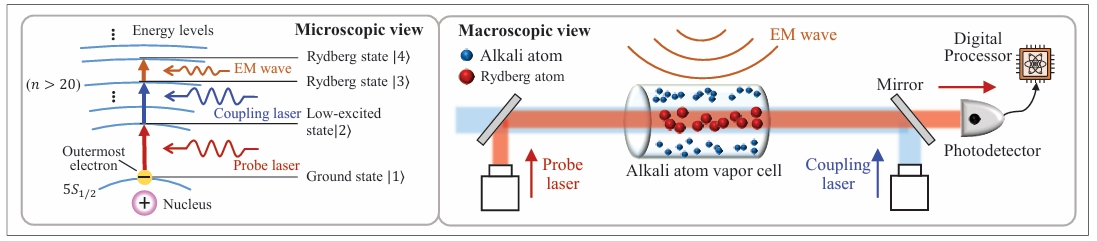
\includegraphics[width=0.92\textwidth]{rare_setup.png}\\[-1pt]
  {\tiny Microscopic (four-level excitation) and macroscopic (vapour cell) view. Adapted from~\cite{cui2026rare}.}
\end{center}
\vspace{-1mm}
\begin{columns}[T]
\column{0.48\textwidth}
\begin{tcolorbox}[mybox]
  \small\textbf{Conventional antenna receivers}
  \begin{itemize}\footnotesize\setlength\itemsep{1pt}
    \item Antenna size $\approx\lambda/2$ ($\approx1.5$~m at 100~MHz)
    \item Front-end thermal noise ($-174$~dBm/Hz)
    \item One resonant antenna and RF chain per band
    \item Weak-field sensitivity limited by the antenna aperture and receiver noise
  \end{itemize}
\end{tcolorbox}
\column{0.48\textwidth}
\begin{tcolorbox}[mybox]
  \small\textbf{Rydberg atomic receivers}
  \begin{itemize}\footnotesize\setlength\itemsep{1pt}
    \item Rydberg atoms ($n>20$): size $\propto n^2$, very large dipole moment
    \item Probe $|1\rangle\!\to\!|2\rangle$, coupling $|2\rangle\!\to\!|3\rangle$, RF $|3\rangle\!\leftrightarrow\!|4\rangle$
    \item RF field read optically from probe transmission (EIT/AT)
    \item $\sim$1~cm cell for any carrier; band set by the choice of Rydberg levels
  \end{itemize}
\end{tcolorbox}
\end{columns}
\end{frame}

%% ---- 4. Literature survey -----------------------------
\begin{frame}{Literature Survey}
\small
\renewcommand{\arraystretch}{1.3}
\begin{tabular}{>{\raggedright\arraybackslash}p{3.4cm}>{\raggedright\arraybackslash}p{3.4cm}>{\raggedright\arraybackslash}p{7.2cm}}
\toprule
\textbf{Work} & \textbf{Focus} & \textbf{Key contribution}\\
\midrule
Cui \textit{et al.}, 2024 (arXiv)~\cite{cui2026rare} & Overview of RAREs & Architecture, sensitivity and bandwidth; multi-band reception; open problems incl.\ channel estimation\\
\addlinespace[6pt]
Chen \textit{et al.}, 2025~\cite{chen2025harnessing} & LO-free and LO-dressed receivers & SNR, MI, SER and distortion regions from the Lindblad model (QuTiP)\\
\addlinespace[6pt]
Cui \textit{et al.}, 2025 (JSAC)~\cite{cui2025towards} & Atomic MIMO & Biased phase-retrieval model; biased GS \\
\addlinespace[6pt]
Xu \textit{et al.}, 2025~\cite{xu2025channel} & Channel estimation & Taylor linearisation; GD (1D), PGD with rank-$L_k$ SVD (2D); CRLB\\
\bottomrule
\end{tabular}

\vspace{4mm}
\footnotesize\textbf{Receiver models used in the literature}
\begin{itemize}\footnotesize\setlength\itemsep{2pt}
  \item \textbf{LO-free and LO-dressed models}~\cite{chen2025harnessing}
  \item \textbf{Magnitude-only measurement model}~\cite{cui2025towards}
  \item \textbf{Linear model}: magnitude model with a strong reference, linearised by a first-order Taylor expansion~\cite{xu2025channel}
\end{itemize}
\end{frame}

%% =========================================================
%% PART A: Chen et al.
%% =========================================================

%% ---- 5. Four-level model + setup -------------------------
\begin{frame}{Part A~\cite{chen2025harnessing}: Four-Level Model and Simulation Setup}
\begin{columns}[T]
\column{0.55\textwidth}
\footnotesize
\setlength{\abovedisplayskip}{3pt}\setlength{\belowdisplayskip}{3pt}
\setlength{\abovedisplayshortskip}{3pt}\setlength{\belowdisplayshortskip}{3pt}
\textcolor{mainblue}{\textbf{Energy levels (Cs)}}\\[1pt]
$|1\rangle{=}6S_{1/2}\to|2\rangle{=}6P_{3/2}\to|3\rangle{=}47D_{5/2}\to|4\rangle{=}48P_{3/2}$;
probe $\Omega_p$, coupling $\Omega_c$, RF $\Omega$

\vspace{3mm}
\textcolor{mainblue}{\textbf{Hamiltonian of the four-level atom}}
{\setlength{\arraycolsep}{3pt}
\[
  \mathbf H=\frac{\hbar}{2}
  \begin{bmatrix}
  0 & \Omega_p & 0 & 0\\
  \Omega_p & -2\Delta_p & \Omega_c & 0\\
  0 & \Omega_c & -2(\Delta_p{+}\Delta_c) & \Omega\\
  0 & 0 & \Omega & -2(\Delta_p{+}\Delta_c{+}\Delta_{RF})
  \end{bmatrix}
\]}

\vspace{1mm}
\textcolor{mainblue}{\textbf{Lindblad master equation}} (steady state solved in QuTiP~5.3~\cite{johansson2012qutip})
\[
  \dot{\bm\rho}=-\tfrac{j}{\hbar}[\mathbf H,\bm\rho]+\mathcal L(\bm\rho)=0
\]

\vspace{1mm}
\textcolor{mainblue}{\textbf{Probe power at the photodetector}}
\[
  P_{out}=P_{in}\,e^{-k_pL\,\mathrm{Im}(\chi)}
\]

\vspace{2mm}
\begin{center}
\fbox{$\mathbf H\;\to\;\text{Lindblad equation}\;\to\;\bm\rho\;\to\;\rho_{21}\;\to\;\chi\;\to\;P_{out}$}
\end{center}

\column{0.42\textwidth}
\vspace{0.8mm}
\footnotesize
\renewcommand{\arraystretch}{1.25}
\begin{tabular}{ll}
\toprule
\textbf{Parameter} & \textbf{Value}\\
\midrule
$L$, $N_0$ & 1~cm, $10^{15}$~m$^{-3}$\\
$\Omega_p/2\pi$, $\Omega_c/2\pi$ & 8~MHz, 1~MHz\\
$\lambda_p$, beam diam. & 852~nm, 0.76~mm\\
$P_{in}$ & 39.08~$\mu$W\\
$\Omega_{LO}/2\pi$, $\Delta f$ & 4.23~MHz, 150~kHz\\
$f_{RF}$, $B$ & 3.5~GHz, 1~MHz\\
$R_L$, $D$ & 50~$\Omega$, 0.55~A/W\\
$\sigma_{BGN}$, $T$ & $-90$~dBm, 290~K\\
\bottomrule
\end{tabular}\\[3pt]
{\tiny Parameters from Sections IV--V of~\cite{chen2025harnessing}.}

\vspace{1mm}
\setlength{\abovedisplayskip}{2pt}\setlength{\belowdisplayskip}{2pt}
\textcolor{mainblue}{\textbf{RF Rabi frequency}}
\[
  \Omega_{RF}=\frac{\wp_{RF}\,|E_{RF}|}{\hbar}
\]
\textcolor{mainblue}{\textbf{Probe input power}} (beam diameter $d$)
\[
  P_{in}=\frac{\pi}{2\eta_0}\left(\frac{d\,\hbar\,\Omega_p}{2\sqrt{\wp_{12}}}\right)^{2}
\]
{\scriptsize $\wp_{12}=(2.5\,ea_0)^2$, $\wp_{RF}=1443.46\,ea_0$, $\eta_0=377~\Omega$}
\end{columns}
\end{frame}

%% ---- 6. EIT/AT surface -----------------------------------

\begin{frame}{Part A~\cite{chen2025harnessing}: EIT/AT Response of the LO-free Receiver}
\begin{columns}[T]
\column{0.55\textwidth}
\begin{center}
  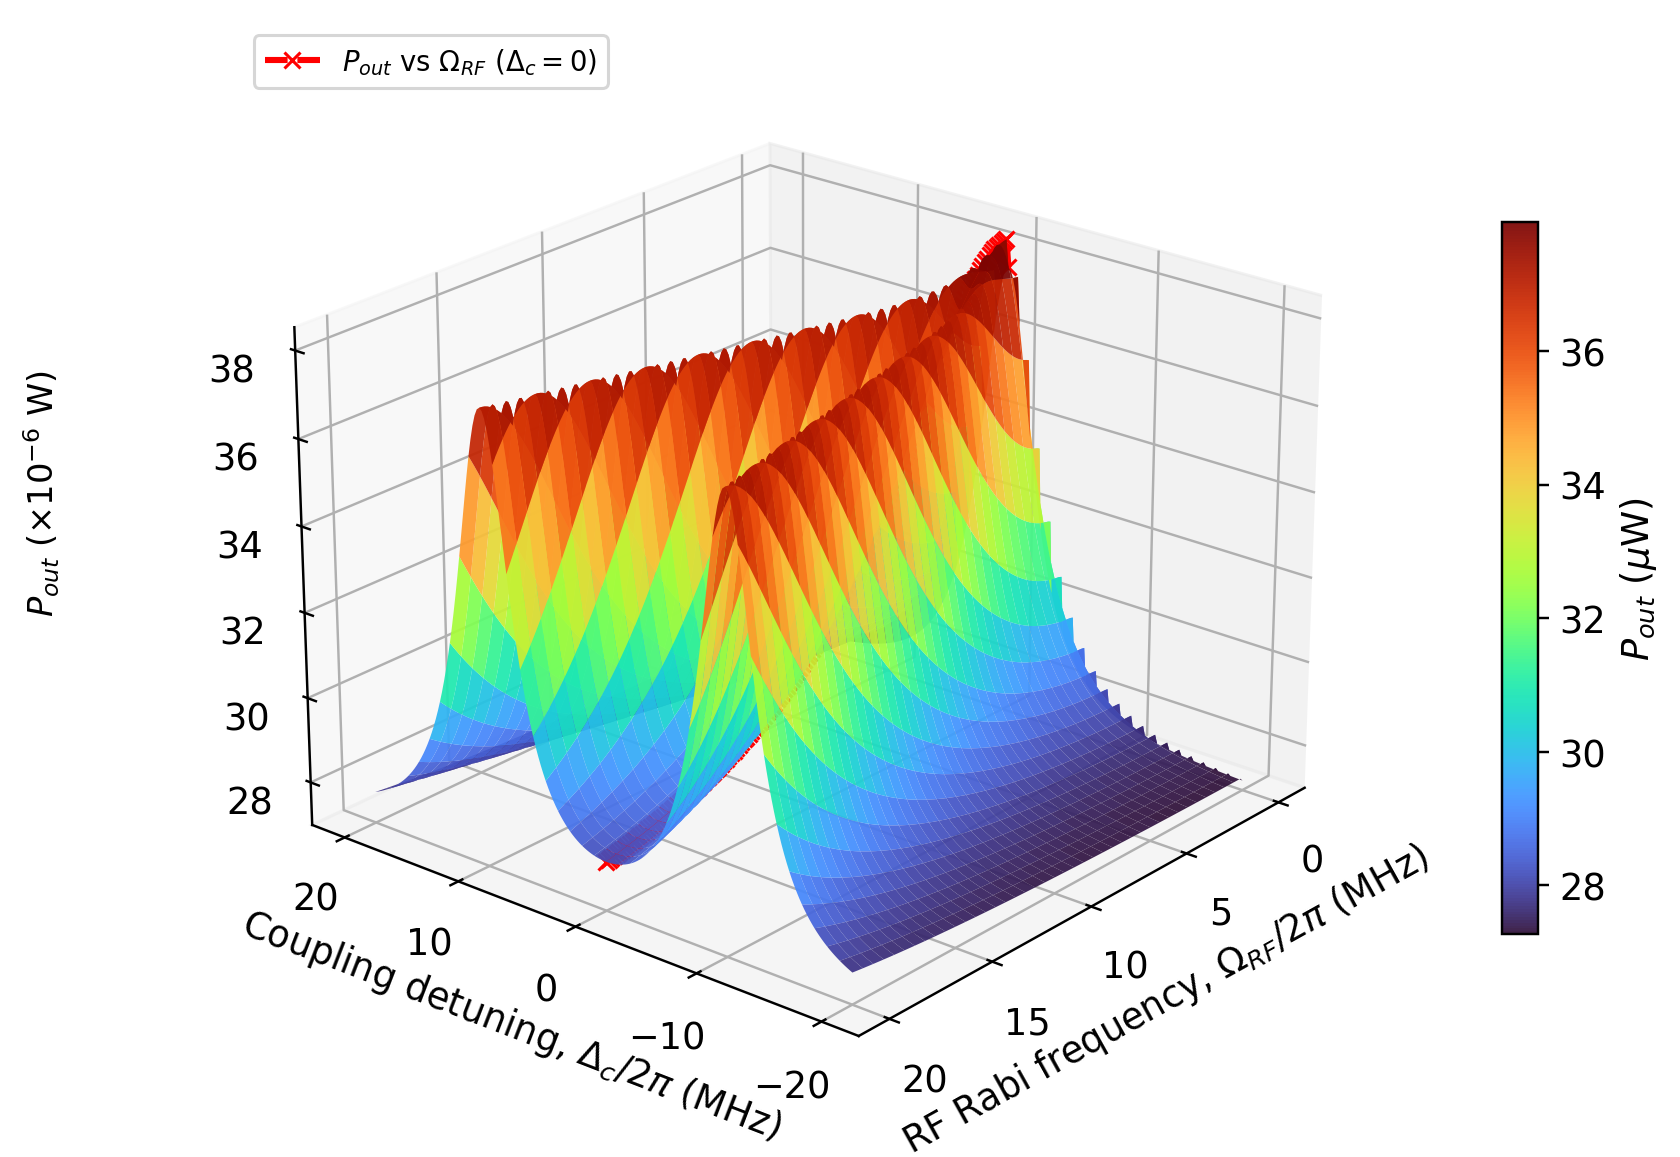
\includegraphics[width=\linewidth,height=0.72\textheight,keepaspectratio]{h_fig3_surface.png}\\
  {\tiny $P_{out}$ versus $\Delta_c$ and $\Omega_{RF}$ (Fig.~3 of~\cite{chen2025harnessing})}
\end{center}
\column{0.42\textwidth}
\footnotesize
\textbf{Graph generation}
\begin{itemize}\setlength\itemsep{1pt}
  \item Grid of $(\Delta_c,\Omega_{RF})$; at each point build $\mathbf H$
  \item QuTiP steady state $\to\rho_{21}\to\chi\to P_{out}$
  \item $P_{out}=P_{in}\,e^{-k_pL\,\mathrm{Im}(\chi)}$, with $\chi=C_0\rho_{21}$
\end{itemize}
\vspace{2mm}
\textbf{Observations}
\begin{itemize}\setlength\itemsep{2pt}
  \item $\Omega_{RF}=0$: coupling laser opens a transparency window (EIT) at $\Delta_c=0$
  \item RF field couples $|3\rangle\leftrightarrow|4\rangle$ and splits the peak into two AT peaks separated by $\Omega_{RF}$
  \item Red line: transmission at $\Delta_c=0$ falls as $\Omega_{RF}$ grows
  \item Peak $P_{out}=38.3~\mu$W
\end{itemize}
\end{columns}
\end{frame}

%% ---- 7. Slices + distortion ------------------------------
\begin{frame}{Part A~\cite{chen2025harnessing}: EIT/AT Spectra and Distortion Region (LO-free)}
\begin{columns}[T]
\column{0.53\textwidth}
\begin{center}
  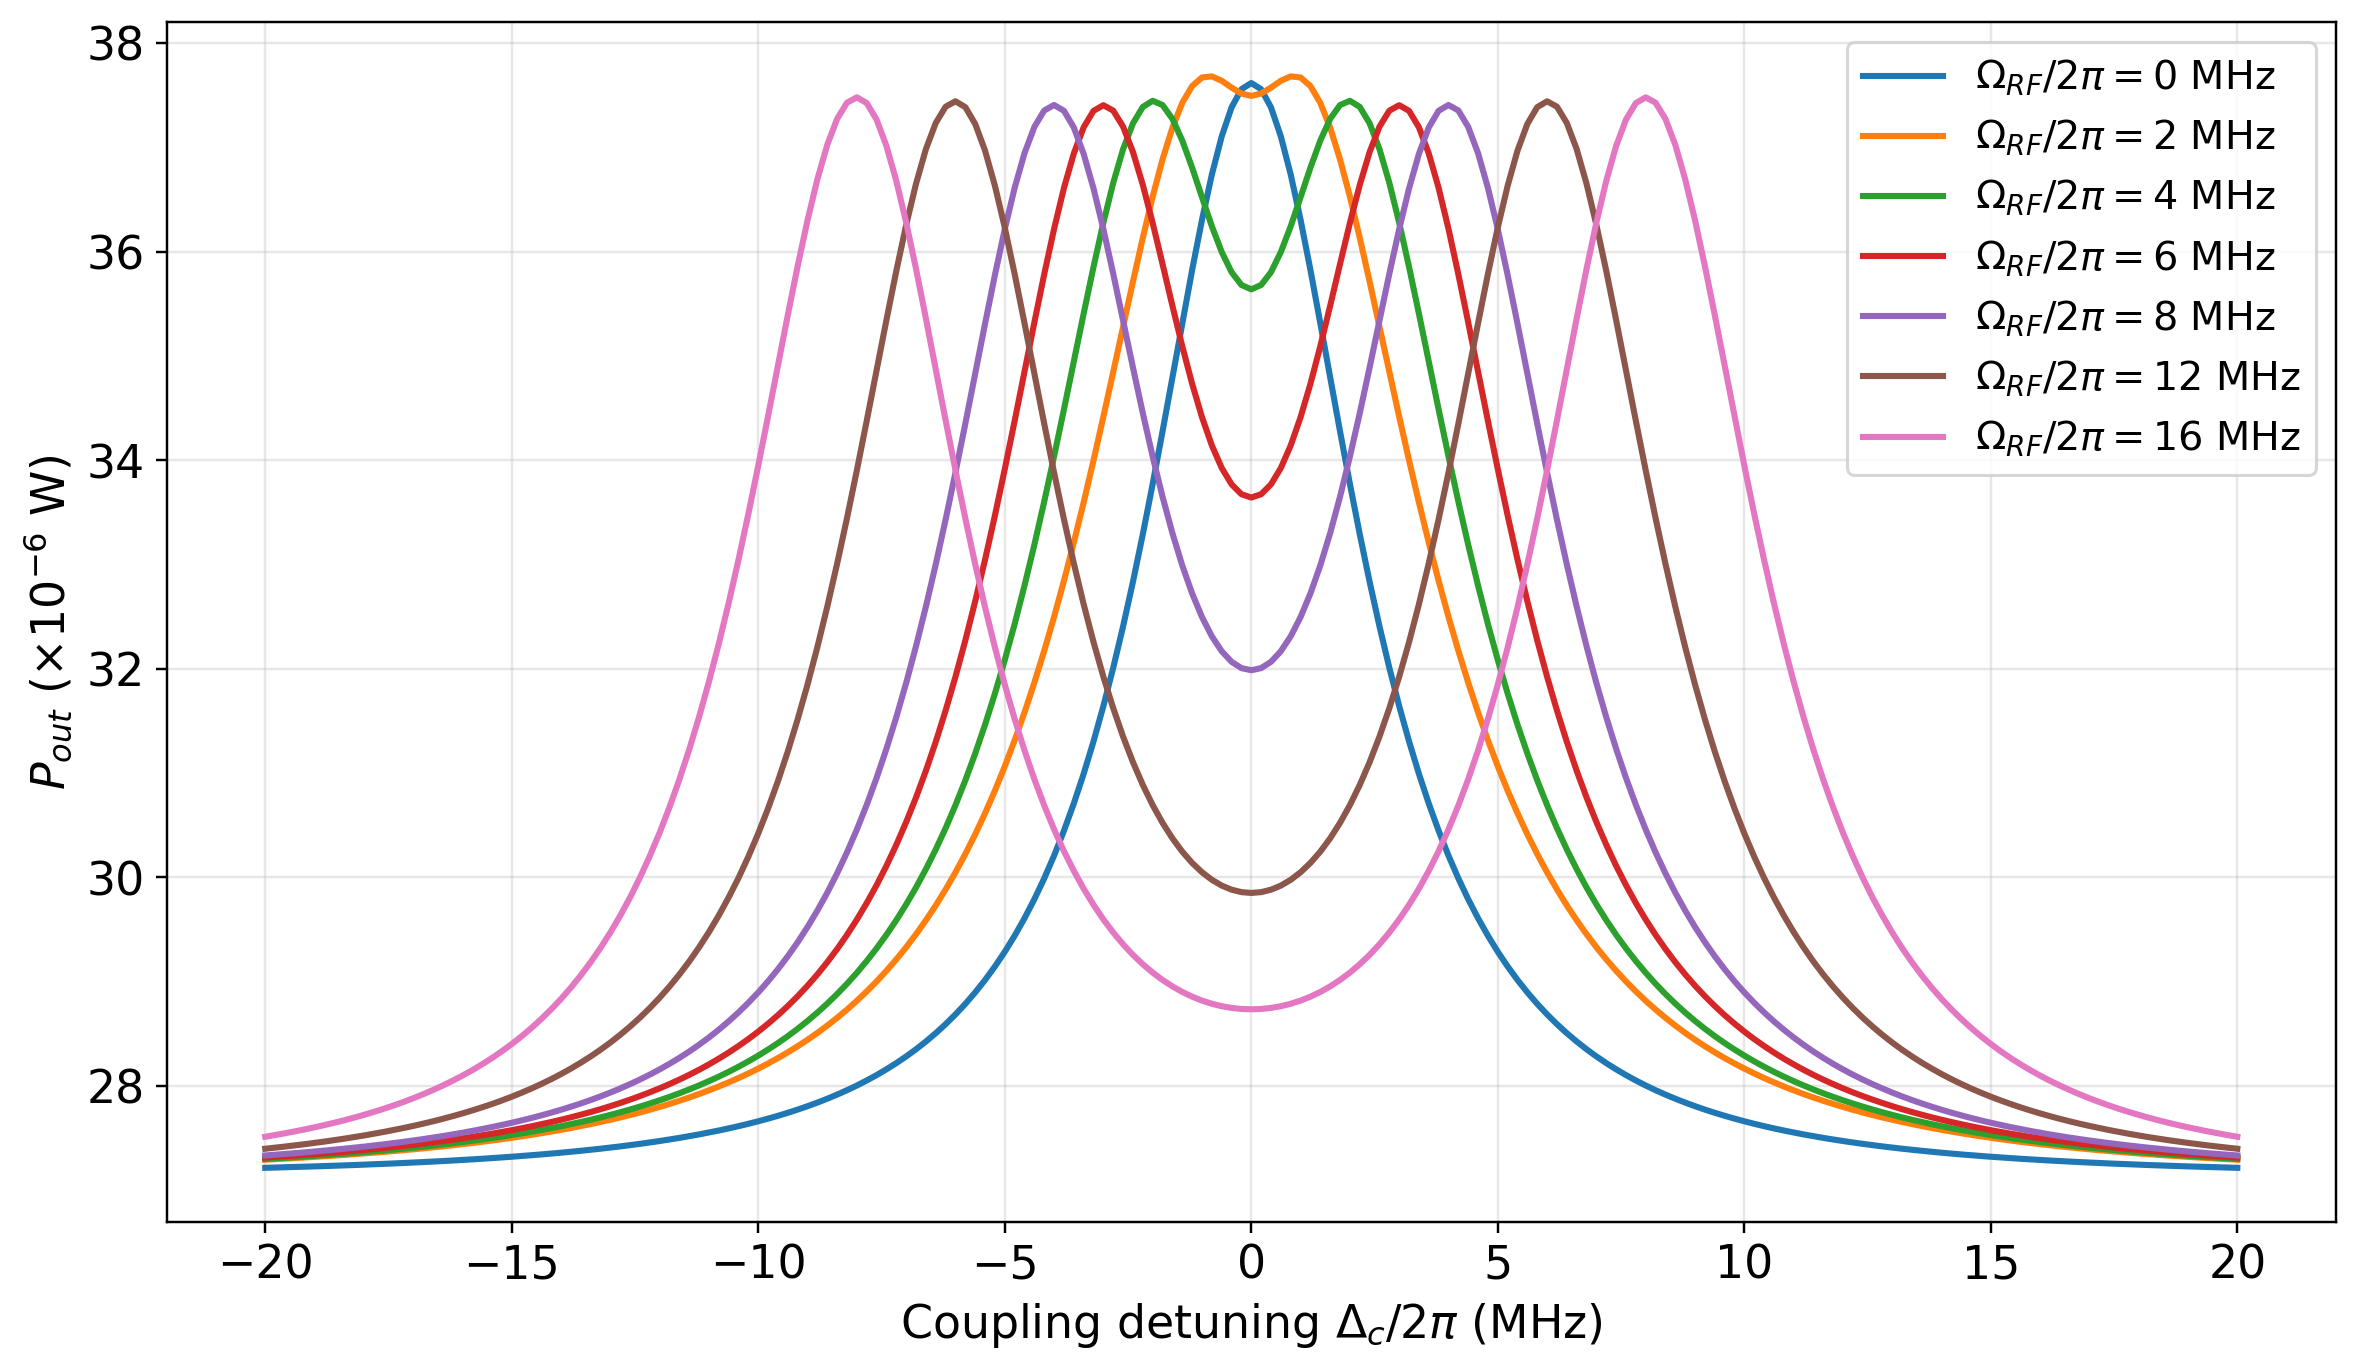
\includegraphics[width=\linewidth,height=0.46\textheight,keepaspectratio]{h_fig3_slices.png}\\
  {\tiny Spectra at fixed $\Omega_{RF}$ (rows of the surface)}
\end{center}
\column{0.44\textwidth}
\begin{center}
  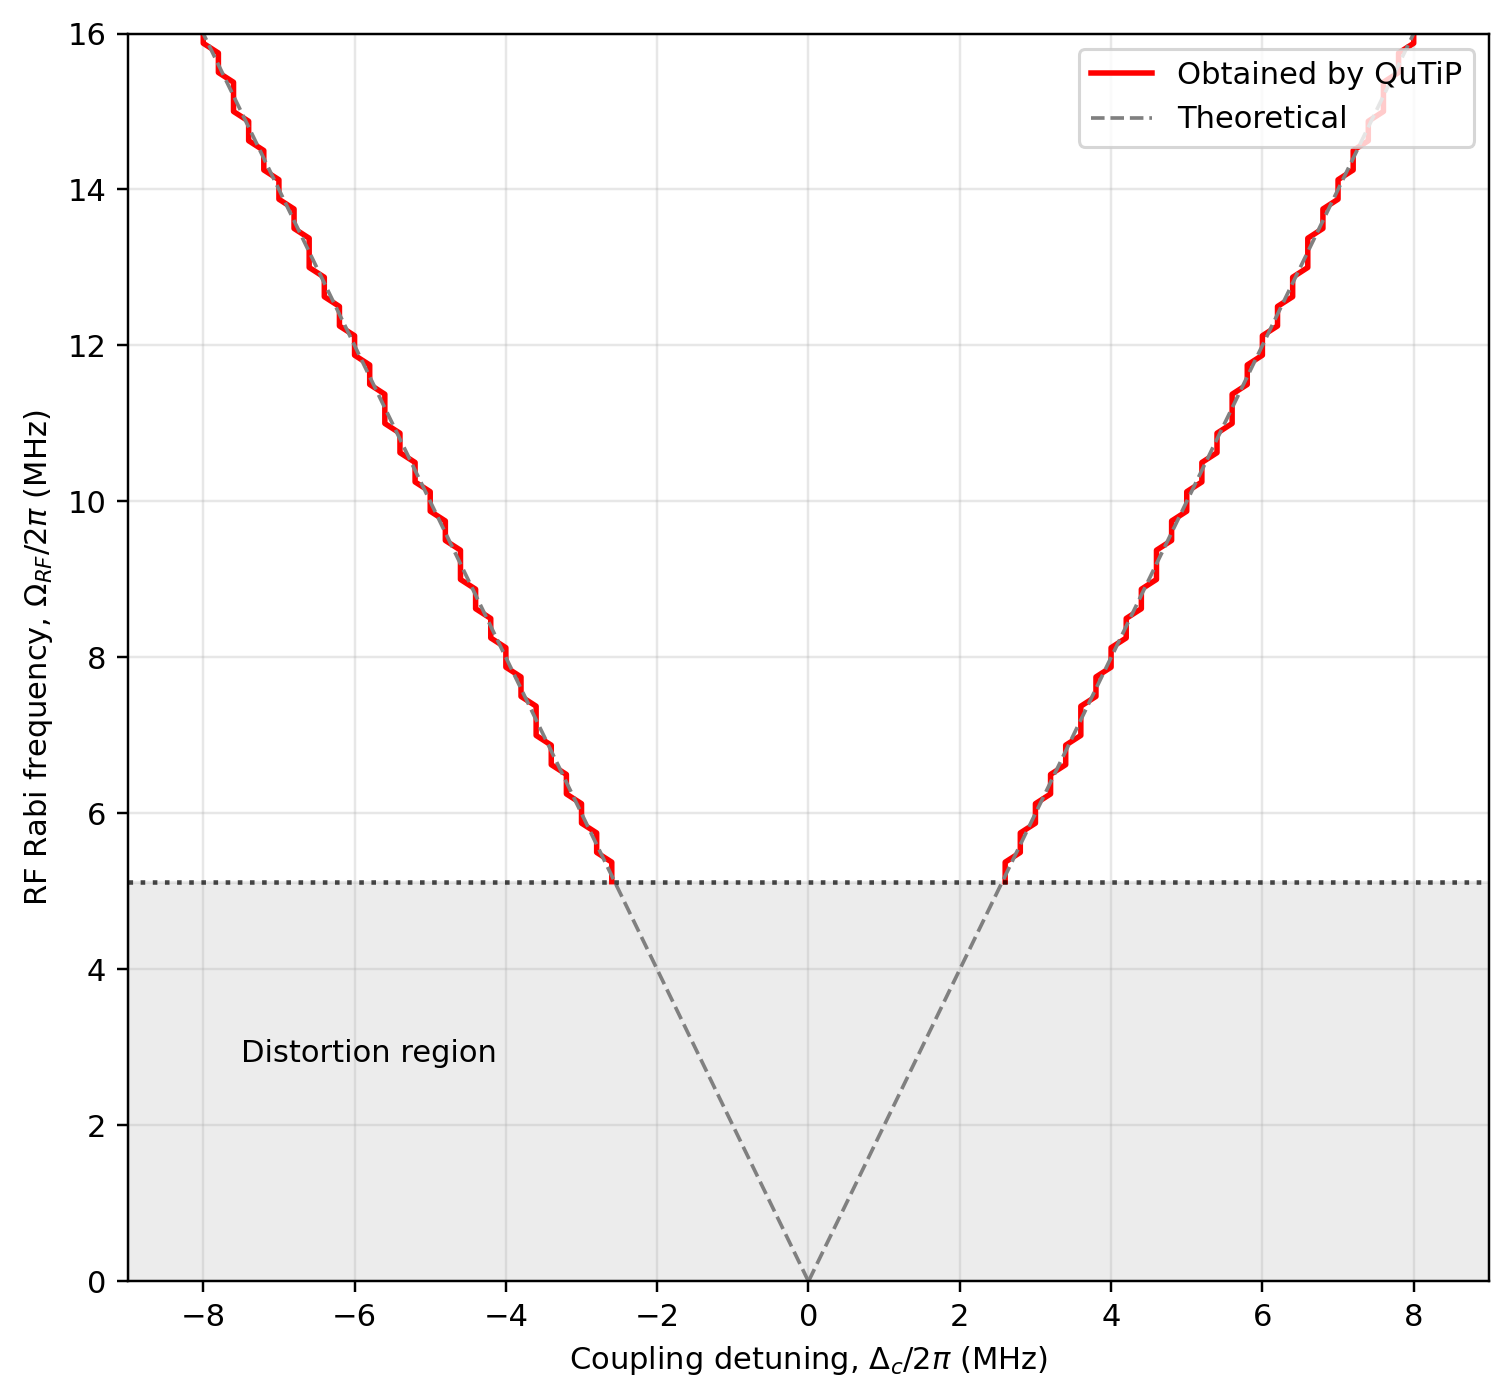
\includegraphics[width=\linewidth,height=0.46\textheight,keepaspectratio]{h_fig4_distortion.png}\\
  {\tiny AT peak positions and distortion region (Fig.~4 of~\cite{chen2025harnessing})}
\end{center}
\end{columns}
\vspace{1mm}
\footnotesize
\begin{itemize}\setlength\itemsep{2pt}
  \item \textbf{Graph generation:} surface data (no new solution) $\to$ two AT peaks in each row $\to$ peak
        separation $\to$ compare with EIT linewidth (FWHM $5.19$~MHz) $\to$ threshold $\Omega_{RF,th}$
  \item Above the threshold the peaks follow $\Delta_c=\pm\Omega_{RF}/2$
  \item Below $\Omega_{RF}/2\pi=5.125$~MHz the peaks merge and $\Omega_{RF}$ cannot be read: distortion region (paper $\approx5.5$~MHz)
\end{itemize}
\end{frame}

%% ---- 8. LO-dressed ---------------------------------------
\begin{frame}{Part A~\cite{chen2025harnessing}: LO-dressed Receiver and Linear Dynamic Range}
\begin{columns}[T]
\column{0.52\textwidth}
\begin{center}
  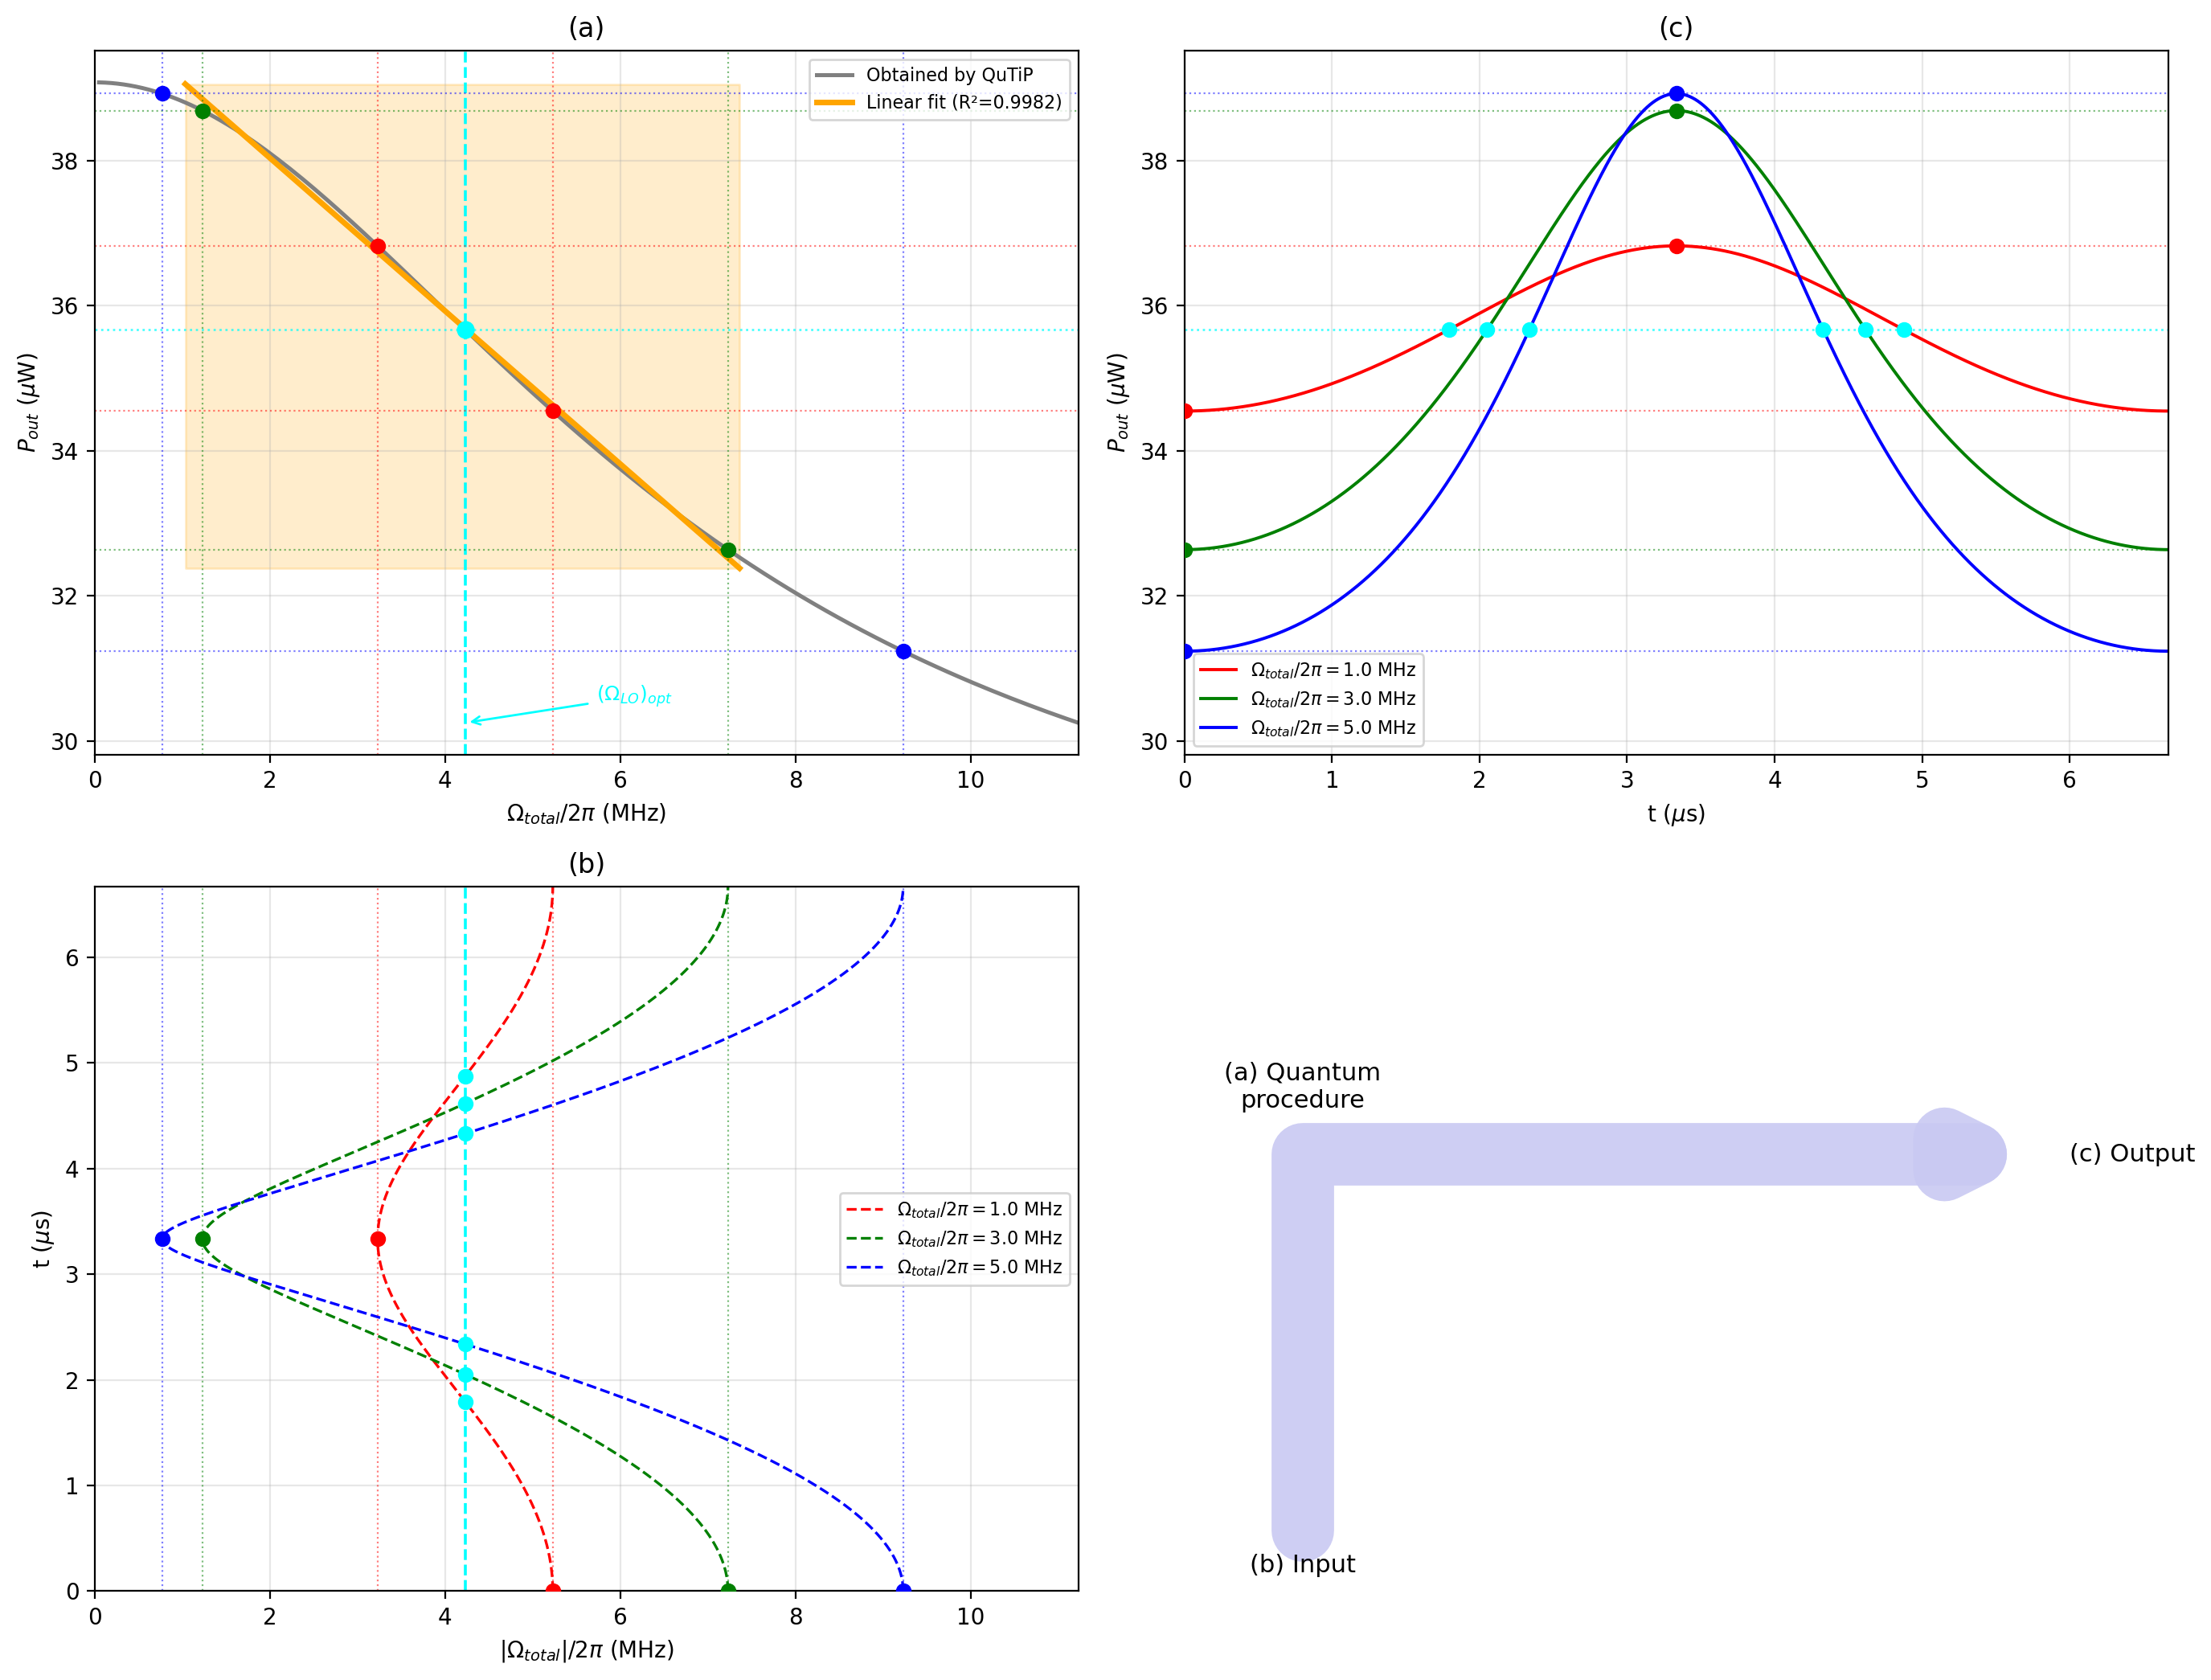
\includegraphics[width=\linewidth,height=0.72\textheight,keepaspectratio]{h_fig5_lodressed.png}\\
  {\tiny (a) $P_{out}$ vs $\Omega_{total}$, (b) input, (c) output (Fig.~5 of~\cite{chen2025harnessing})}
\end{center}
\column{0.45\textwidth}
\footnotesize
\textbf{Model} (atoms act as a mixer, $\Omega_{RF}\ll\Omega_{LO}$)
\[
  \Omega_{total}(t)=\big|\Omega_{LO}+e^{j(2\pi\Delta f t+\Delta\phi)}\Omega_{RF}\big|
\]
\[
  P_{out}(t)\approx\bar P_0+\kappa\,\Omega_{RF}\cos(2\pi\Delta f t+\Delta\phi)
\]
\textbf{Graph generation}
\begin{itemize}\setlength\itemsep{1pt}
  \item (a) $\Omega_{total}$ grid $\to$ QuTiP ($\gamma_3{=}\gamma_4{=}0$) $\to P_{out}(\Omega_{total})$ $\to$ linear fit ($R^2\geq0.998$) $\to\kappa$
  \item (b) $\Omega_{RF},\Delta f\to\Omega_{total}(t)$
  \item (c) $\Omega_{total}(t)\to$ curve (a) $\to P_{out}(t)$
\end{itemize}
\vspace{1mm}
\textbf{Observations}
\begin{itemize}\setlength\itemsep{1pt}
  \item Linear range $[1.03,7.36]$~MHz (paper $\approx[1.3,7.2]$)

\end{itemize}
\end{columns}
\end{frame}



%% =========================================================
%% PART B: Xu et al.
%% =========================================================

%% ---- 10. Atomic MIMO model -------------------------------
\begin{frame}{Part B~\cite{xu2025channel}: Atomic MIMO Model and Linearisation}
\vspace*{-4mm}
\begin{columns}[T]
\column{0.50\textwidth}
\footnotesize
\setlength{\abovedisplayskip}{3pt}\setlength{\belowdisplayskip}{3pt}
\textbf{Measurement at cell $i$, pilot slot $p$}~\cite{cui2025towards,xu2025channel}
\[
  y_{i,p}=\Big|\sum_{k=1}^K g_{i,k}s_{k,p}+b_{i,p}+n_{i,p}\Big|
\]
\textbf{User channel} ($L_k$ paths)
\[
  g_{i,k}=\sum_{l=1}^{L_k}\frac{1}{\hbar}\bm\mu_{eg}^T\bm\epsilon_{i,k,l}\,\alpha_{l,k}\,e^{-j(i-1)\varphi_{l,k}}
\]
\textbf{Reference signal} (known, from a nearby source)
\[
  b_{i,p}=\frac{s_{b,p}}{\hbar}\,\alpha_b\,\bm\mu_{eg}^T\bm\epsilon_{b,i}\,e^{-j(i-1)\varphi_b}
\]
\begin{itemize}\setlength\itemsep{1pt}
  \item $n_{i,p}\sim\mathcal{CN}(0,\sigma^2)$; $\bm\epsilon$: polarisation; $\alpha$: path gain
  \item Only the magnitude is measured, so LS/MMSE cannot be used directly
\end{itemize}
\column{0.47\textwidth}
\footnotesize
\setlength{\abovedisplayskip}{3pt}\setlength{\belowdisplayskip}{3pt}
\textbf{First-order linearisation} (if $|b|\gg|a+n|$, $a_{i,p}=\sum_kg_{i,k}s_{k,p}$)
\[
  y_{i,p}\approx|b_{i,p}|+\mathrm{Re}\{e^{-j\angle b_{i,p}}a_{i,p}\}+\bar n_{i,p}
\]
{\scriptsize with $\bar n_{i,p}=\mathrm{Re}\{e^{-j\angle b_{i,p}}n_{i,p}\}\sim\mathcal N(0,\sigma^2/2)$}
\[
  \Longrightarrow\;\mathbf Y=\mathrm{Re}\{\mathbf Z\circ(\mathbf G\mathbf S)\}+|\mathbf B|+\mathbf N,\quad Z_{i,p}=e^{-j\angle b_{i,p}}
\]
{\scriptsize $\mathbf Y,\mathbf N\in\mathbb R^{I\times P}$,\; $\mathbf Z,\mathbf B\in\mathbb C^{I\times P}$,\; $\mathbf G\in\mathbb C^{I\times K}$,\; $\mathbf S\in\mathbb C^{K\times P}$}


\vspace{1mm}
\textbf{Strong-reference condition}
\begin{itemize}\setlength\itemsep{3pt}
  \item Linearisation is valid only if $|b_{i,p}|\gg\big|\sum_k g_{i,k}s_{k,p}+n_{i,p}\big|$
  \item With the given parameters, the reference is weaker than $\big|\sum_k g_{i,k}s_{k,p}+n_{i,p}\big|$ ($\approx-2$~dB), so the linear model does not hold
  \item In the simulations, the reference is scaled to $34$~dB above the user signal

\end{itemize}
\end{columns}
\end{frame}


%% ---- 10b. 2D array model --------------------------------
\begin{frame}{Part B~\cite{xu2025channel}: 2D Antenna Array Model}
\begin{columns}[T]
\column{0.50\textwidth}
\footnotesize
\setlength{\abovedisplayskip}{3pt}\setlength{\belowdisplayskip}{3pt}
\textbf{Channel of user $k$ at cell $(i_1,i_2)$}
\[
  g_{i_1,i_2,k}=\sum_{l=1}^{L_k}\frac{1}{\hbar}\bm\mu_{eg}^T\bm\epsilon_{k,l}\,\alpha_{l,k}\,
  e^{-j[(i_1-1)u_{l,k}+(i_2-1)v_{l,k}]}
\]
{\scriptsize $u_{l,k}=\tfrac{2\pi d_1}{\lambda}\cos\theta_{l,k}$,\; $v_{l,k}=\tfrac{2\pi d_2}{\lambda}\sin\theta_{l,k}\cos\phi_{l,k}$}

\vspace{2mm}
\textbf{Reference signal}
\[
  b_{i_1,i_2,p}=\frac{s_{b,p}}{\hbar}\,\alpha_b\,\bm\mu_{eg}^T\bm\epsilon_{b,i_1,i_2}\,
  e^{-j[(i_1-1)u_b+(i_2-1)v_b]}
\]

\vspace{2mm}
\textbf{Magnitude measurement model}
\[
  y_{i_1,i_2,p}=\Big|\sum_{k=1}^K g_{i_1,i_2,k}s_{k,p}+b_{i_1,i_2,p}+n_{i_1,i_2,p}\Big|
\]

\vspace{2mm}
\textbf{Linearised model} (strong reference, $z_{i_1,i_2,p}=\angle b_{i_1,i_2,p}$)
\[
  \begin{aligned}
  y_{i_1,i_2,p}\approx{}&\mathrm{Re}\Big\{e^{-jz_{i_1,i_2,p}}\sum_{k=1}^K g_{i_1,i_2,k}s_{k,p}\Big\}\\
  &+|b_{i_1,i_2,p}|+\bar n_{i_1,i_2,p}
  \end{aligned}
\]

\column{0.47\textwidth}
\vspace{-4mm}
\begin{center}
  \includegraphics[width=0.88\linewidth]{array2d.png}\\[1pt]
  {\tiny Rydberg atom-based 2D antenna array with $K$ users and an LO reference. Adapted from~\cite{xu2025channel}.}
\end{center}
\footnotesize
\setlength{\abovedisplayskip}{3pt}\setlength{\belowdisplayskip}{3pt}
\textbf{Mode-3 unfolded linear model}
\[
  \mathbf Y_{(3)}=\mathrm{Re}\{\mathbf Z_{(3)}\circ(\mathbf S^T\mathbf G_{(3)})\}+|\mathbf B_{(3)}|+\mathbf N_{(3)}
\]
\vspace{1em}
{\scriptsize $\mathbf Y_{(3)},\mathbf N_{(3)}\in\mathbb R^{P\times I_1I_2}$,\; $\mathbf Z_{(3)},\mathbf B_{(3)}\in\mathbb C^{P\times I_1I_2}$\\
$\mathbf S\in\mathbb C^{K\times P}$,\; $\mathbf G_{(3)}\in\mathbb C^{K\times I_1I_2}$}
\end{columns}
\end{frame}

%% ---- 11. GD + GS -----------------------------------------
\begin{frame}{Part B~\cite{xu2025channel}: GD and Biased GS Algorithms (1D Array)}
\begin{columns}[T]
\column{0.49\textwidth}
\small\textbf{Gradient descent (GD)}~\cite{xu2025channel}\\[2pt]
\footnotesize
Cost:\;
$\mathcal L(\mathbf G)=\big\|\mathbf Y-|\mathbf B|-\mathrm{Re}\{\mathbf Z\circ(\mathbf G\mathbf S)\}\big\|_F^2$
\vspace{1mm}
\begin{algorithmic}[1]
\Require $\mathbf Y$, $\mathbf S$, $\mathbf Z$, $\mathbf B$, $\mathbf G^0$, $T_{\max}$, $\epsilon$
\State $t=0$
\Repeat
  \State $\hat{\mathbf Y}^t=\mathrm{Re}\{\mathbf Z\circ(\mathbf G^t\mathbf S)\}+|\mathbf B|$
  \State $\mathbf E^t=\mathbf Y-\hat{\mathbf Y}^t$
  \State $\mathbf D^t=-2\,(\mathbf E^t\circ\mathbf Z^*)\,\mathbf S^H$
  \State $\mathbf G^{t+1}=\mathbf G^t-\eta_t\mathbf D^t$,\quad $t\gets t+1$
\Until{$\|\mathbf G^{t+1}-\mathbf G^{t}\|_F^2<\epsilon$ \textbf{or} $t\geq T_{\max}$}
\State \Return $\hat{\mathbf G}=\mathbf G^t$
\end{algorithmic}
\vspace{2mm}
\begin{itemize}\setlength\itemsep{1pt}
  \item $\mathbf G^0\sim\mathcal{CN}(0,0.1)$, $T_{\max}=500$, $\epsilon=10^{-8}$; step $\eta_t$: start at 1, halve until $\mathcal L$ decreases
  \item Uses the \textbf{linearised} model, so it inherits the Taylor error
\end{itemize}
\column{0.49\textwidth}
\small\textbf{Biased Gerchberg--Saxton (GS)}~\cite{cui2025towards,netrapalli2015}\\[2pt]
\footnotesize
Model:\;
$\mathbf Y=|\mathbf G\mathbf S+\mathbf B+\mathbf N|$ \;(exact magnitude model)
\vspace{1mm}
\begin{algorithmic}[1]
\Require $\mathbf Y$, $\mathbf S$, $\mathbf B$, $\mathbf G^0$, $T_{\max}$, $\epsilon$
\State $t=0$
\Repeat
  \State $\bm\Theta^t=\angle(\mathbf G^t\mathbf S+\mathbf B)$
         \Comment{phase estimate}
  \State $\mathbf R^t=\mathbf Y\circ e^{j\bm\Theta^t}$
         \Comment{magnitude + phase}
  \State $\mathbf G^{t+1}=(\mathbf R^t-\mathbf B)\,\mathbf S^H(\mathbf S\mathbf S^H)^{-1}$
         \Comment{LS}
  \State $t\gets t+1$
\Until{$\|\mathbf G^{t+1}-\mathbf G^{t}\|_F^2<\epsilon$ \textbf{or} $t\geq T_{\max}$}
\State \Return $\hat{\mathbf G}=\mathbf G^t$
\end{algorithmic}
\vspace{2mm}
\begin{itemize}\setlength\itemsep{1pt}
  \item $\mathbf G^0$: initial channel estimate (spectral initialisation), $T_{\max}=100$
  \item Works on the \textbf{exact} magnitude model; no rank structure (1D only)
\end{itemize}
\end{columns}
\end{frame}

%% ---- 12. PGD + CRLB --------------------------------------
\begin{frame}{Part B~\cite{xu2025channel}: PGD Algorithm (2D Array) and CRLB}
\begin{columns}[T]
\column{0.49\textwidth}
\small\textbf{Projected gradient descent (PGD)}\\[2pt]
\footnotesize
Channel tensor unfolded along mode 3: $\mathbf G_{(3)}\in\mathbb C^{K\times I_1I_2}$
\vspace{1mm}
\begin{algorithmic}[1]
\Require $\mathbf Y_{(3)}$, $\mathbf Z_{(3)}$, $\mathbf B_{(3)}$, $\mathbf S$, $\{L_k\}$, $\mathbf G^0_{(3)}$, $T_{\max}$, $\epsilon$
\State $t=0$
\Repeat
  \State $\mathbf E^t=\mathbf Y_{(3)}-|\mathbf B_{(3)}|-\mathrm{Re}\{\mathbf Z_{(3)}\circ(\mathbf S^T\mathbf G^t_{(3)})\}$
  \State $\nabla f=-\mathbf S^*(\mathbf E^t\circ\mathbf Z^*_{(3)})$
  \State $\mathbf M=\mathbf G^t_{(3)}-\zeta\,\nabla f$
         \Comment{gradient step}
  \For{$k=1,\dots,K$}
         \Comment{projection}
    \State reshape $[\mathbf M]_{k,:}$ to $I_1\times I_2$, SVD, keep $L_k$ largest singular values $\to[\mathbf G^{t+1}_{(3)}]_{k,:}$
  \EndFor
  \State $t\gets t+1$
\Until{$\|\mathbf G^{t+1}_{(3)}-\mathbf G^{t}_{(3)}\|_F^2<\epsilon$ \textbf{or} $t\geq T_{\max}$}
\State \Return $\hat{\mathbf G}_{(3)}=\mathbf G^t_{(3)}$
\end{algorithmic}
\vspace{1mm}
\begin{itemize}\setlength\itemsep{1pt}
  \item $\mathbf G^0_{(3)}\sim\mathcal{CN}(0,0.1)$, $T_{\max}=300$
  \item Each path gives a rank-one outer product, so rank $\leq L_k$

\end{itemize}
\column{0.49\textwidth}
\small\textbf{CRLB derivation}~\cite{xu2025channel}\\[2pt]
\footnotesize
\begin{itemize}\setlength\itemsep{3pt}
  \item Vectorised linear model, $\mathbf g=\mathrm{vec}(\mathbf G)$:\\[2pt]
        $\mathbf y=\mathrm{Re}\{\mathbf z\circ(\mathbf I\otimes\mathbf S^T)\mathbf g\}+|\mathbf b|+\mathbf n$
  \item Fisher information:
\end{itemize}
\[
  \mathrm{FIM}(\mathbf g)=\tfrac{1}{4\sigma^2}(\mathbf I\otimes\mathbf S^T)^H(\mathbf I\otimes\mathbf S^T)
  =\tfrac{1}{4\sigma^2}\,\mathbf I\otimes(\mathbf S^*\mathbf S^T)
\]
\begin{itemize}
  \item Inverting the FIM:
\end{itemize}
\[
  \mathrm{CRB}(\mathbf g)=4\sigma^2\big[\mathbf I_{I_1I_2}\otimes(\mathbf S^*\mathbf S^T)^{-1}\big]
\]
\begin{itemize}\setlength\itemsep{1pt}
  \item Decreases with SNR ($\propto\sigma^2$) and with pilot length
\end{itemize}
\end{columns}
\end{frame}

%% ---- 13. CE: 1D ------------------------------------------
\begin{frame}{Part B~\cite{xu2025channel}: 1D Array Results}
\begin{columns}[T]
\column{0.56\textwidth}
\begin{center}
  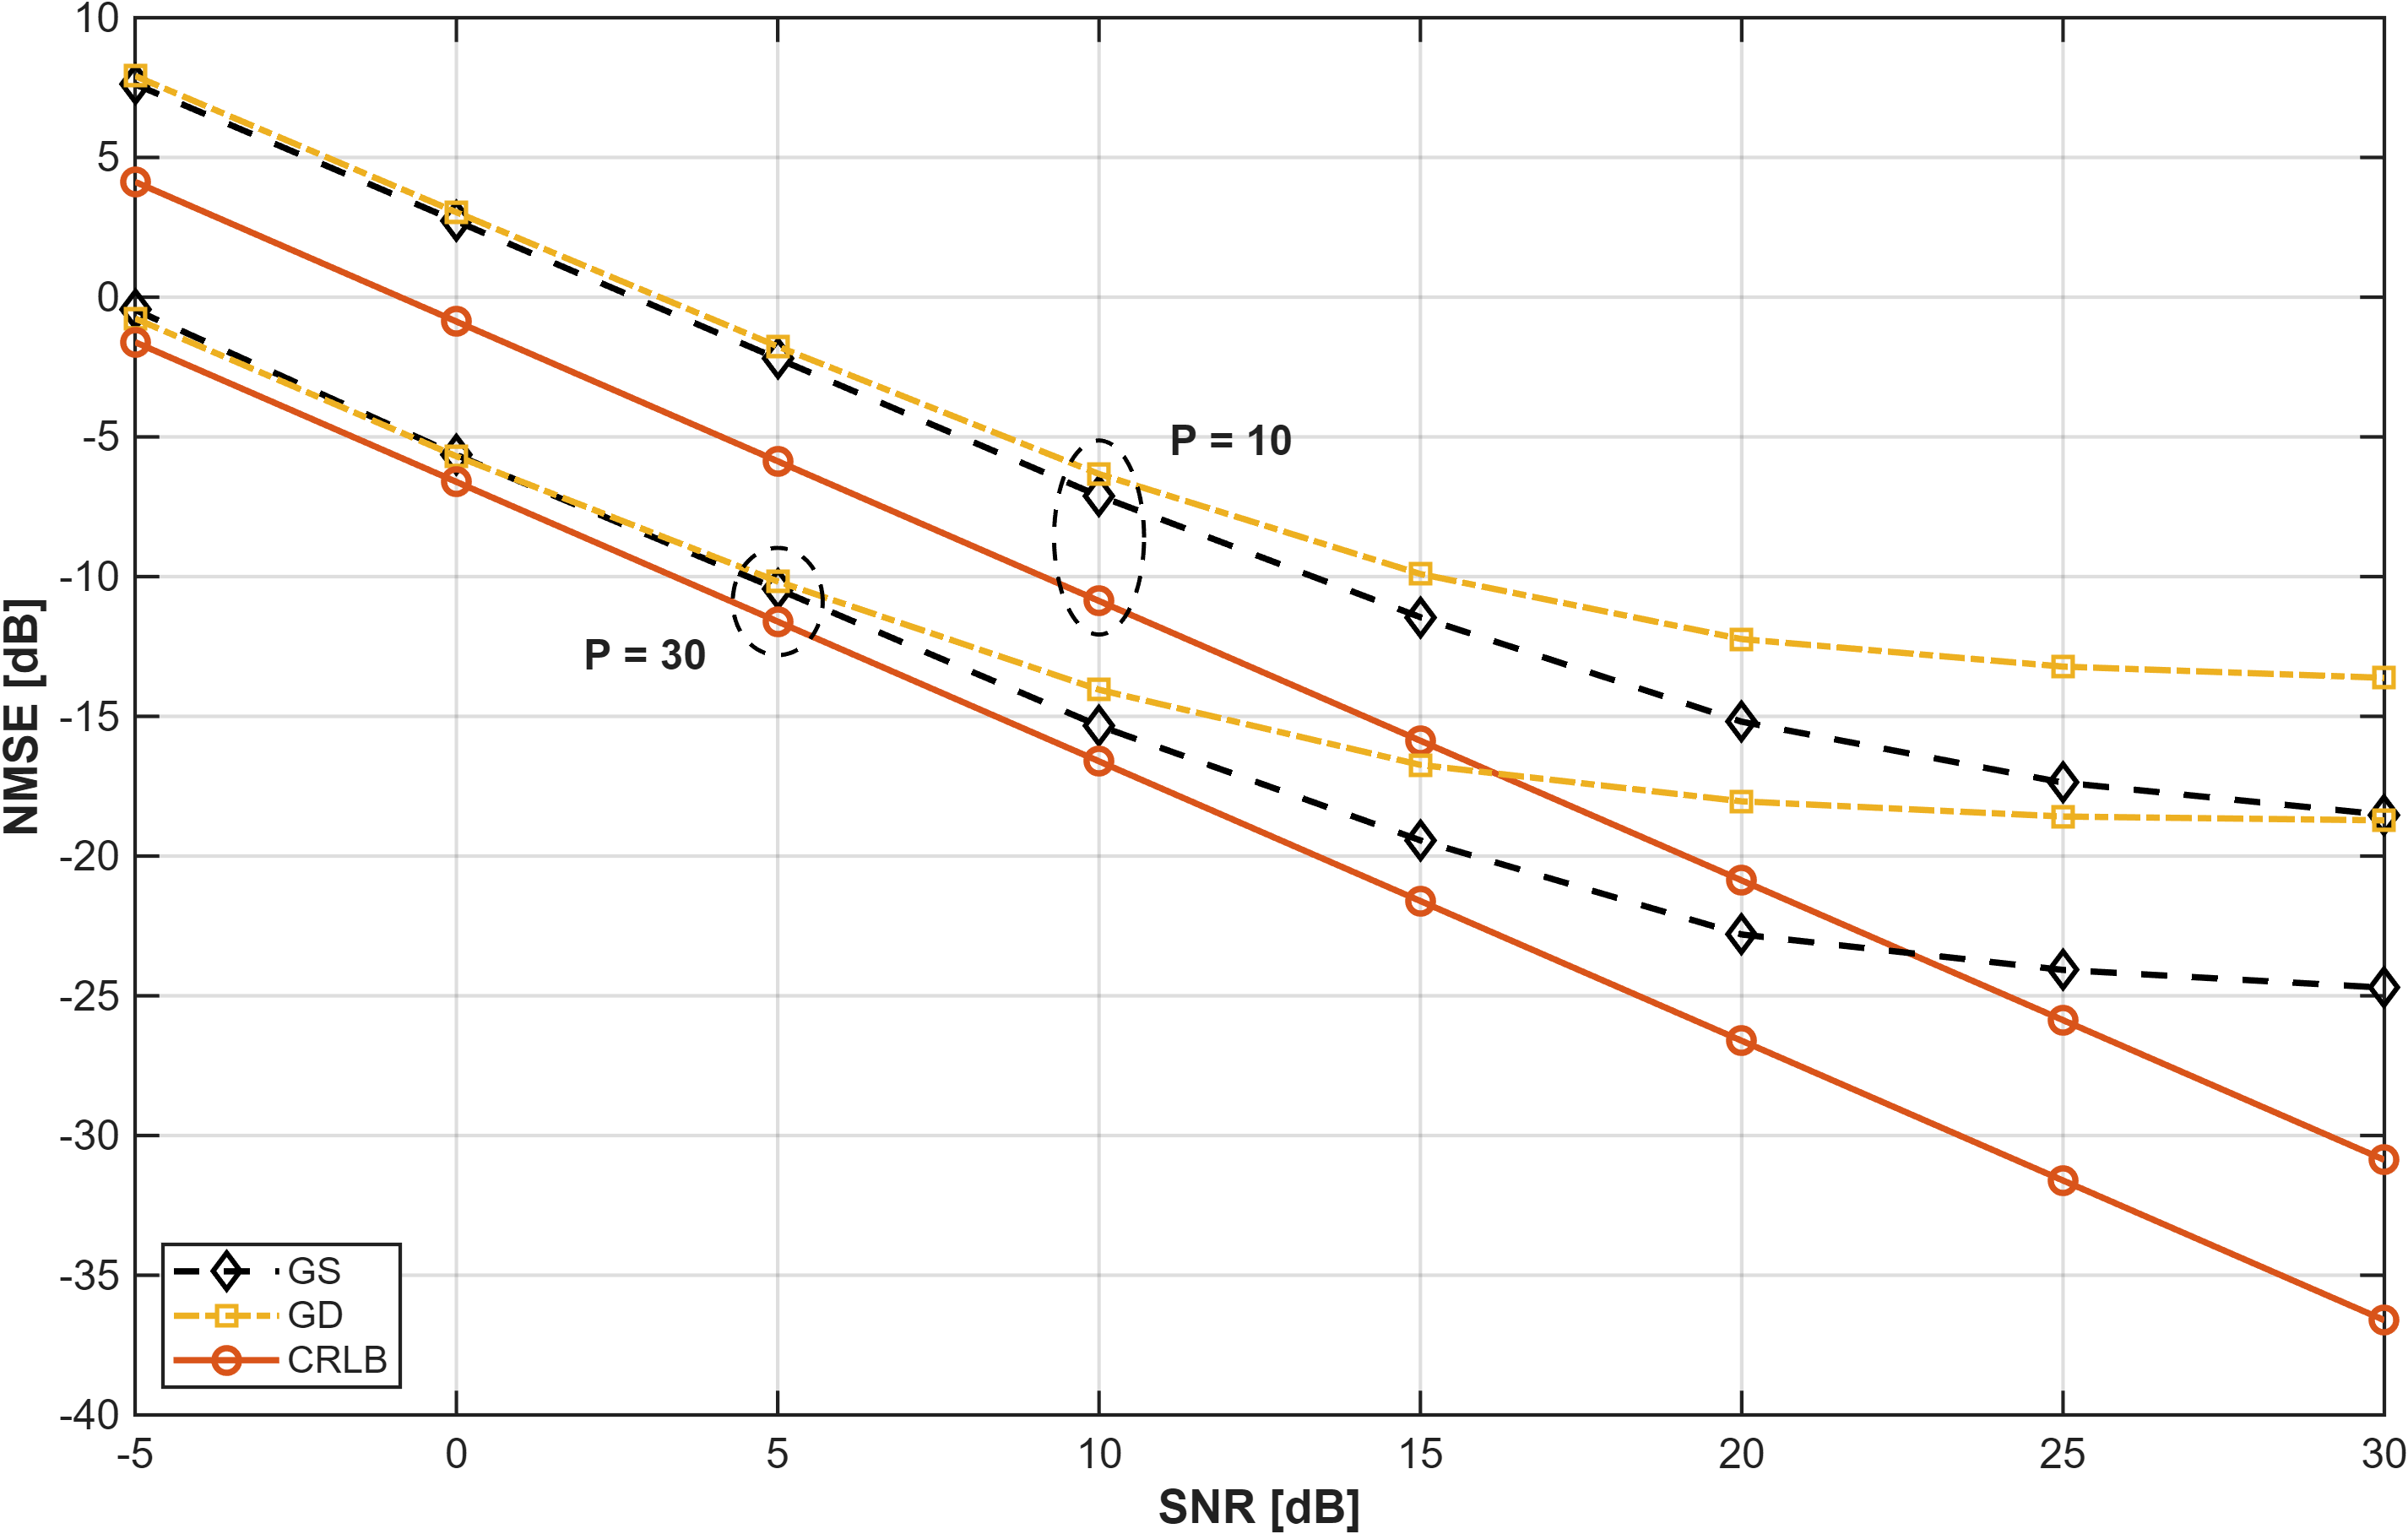
\includegraphics[width=\linewidth,height=0.70\textheight,keepaspectratio]{ce_fig3_1d.png}\\
  {\tiny NMSE vs SNR, 1D array ($I=8$, $K=3$): biased GS, GD, CRLB}
\end{center}
\column{0.41\textwidth}
\footnotesize
\textbf{Setup}
\begin{itemize}\setlength\itemsep{1pt}
  \item $K=3$, $L_k\in\{3,\dots,7\}$, $I=8$ (1D), $8\times8$ (2D)
  \item NMSE $=\sum\|\mathbf G-\hat{\mathbf G}\|_F^2/\sum\|\mathbf G\|_F^2$; 500 Monte Carlo runs
\end{itemize}
\vspace{1mm}
\textbf{Observations}
\begin{itemize}\setlength\itemsep{3pt}
  \item $P=30$: both close to the CRLB at low and medium SNR (at 5~dB: GS $-10.5$, GD $-10.2$, CRLB $-11.6$~dB)
  \item $P=10$: both about 4~dB above the bound
  \item GD flattens at high SNR ($\approx-18.7$~dB, $P=30$): the second-order Taylor term dominates once the noise is small
  \item GS uses the exact model and flattens lower ($-24.7$~dB), so curves for different $P$ can meet at high SNR
\end{itemize}
\vspace{1mm}
\textbf{Strong-reference condition}
\begin{itemize}\setlength\itemsep{2pt}
  \item Dropped term $\sim|a+n|^2/(2|b|)$: accuracy depends on the reference-to-signal ratio
  \item With the paper's parameters, $\mathbb E|b|^2/\mathbb E|a+n|^2\approx-2$~dB: the reference is weaker than the signal
  \item In these simulations the reference is scaled to $\mathbb E|b|^2/\mathbb E|a|^2=34$~dB
\end{itemize}
\end{columns}
\end{frame}

%% ---- 14. CE: 2D + pilots ---------------------------------
\begin{frame}{Part B~\cite{xu2025channel}: 2D Array and Pilot Length}
\begin{columns}[T]
\column{0.49\textwidth}
\begin{center}
  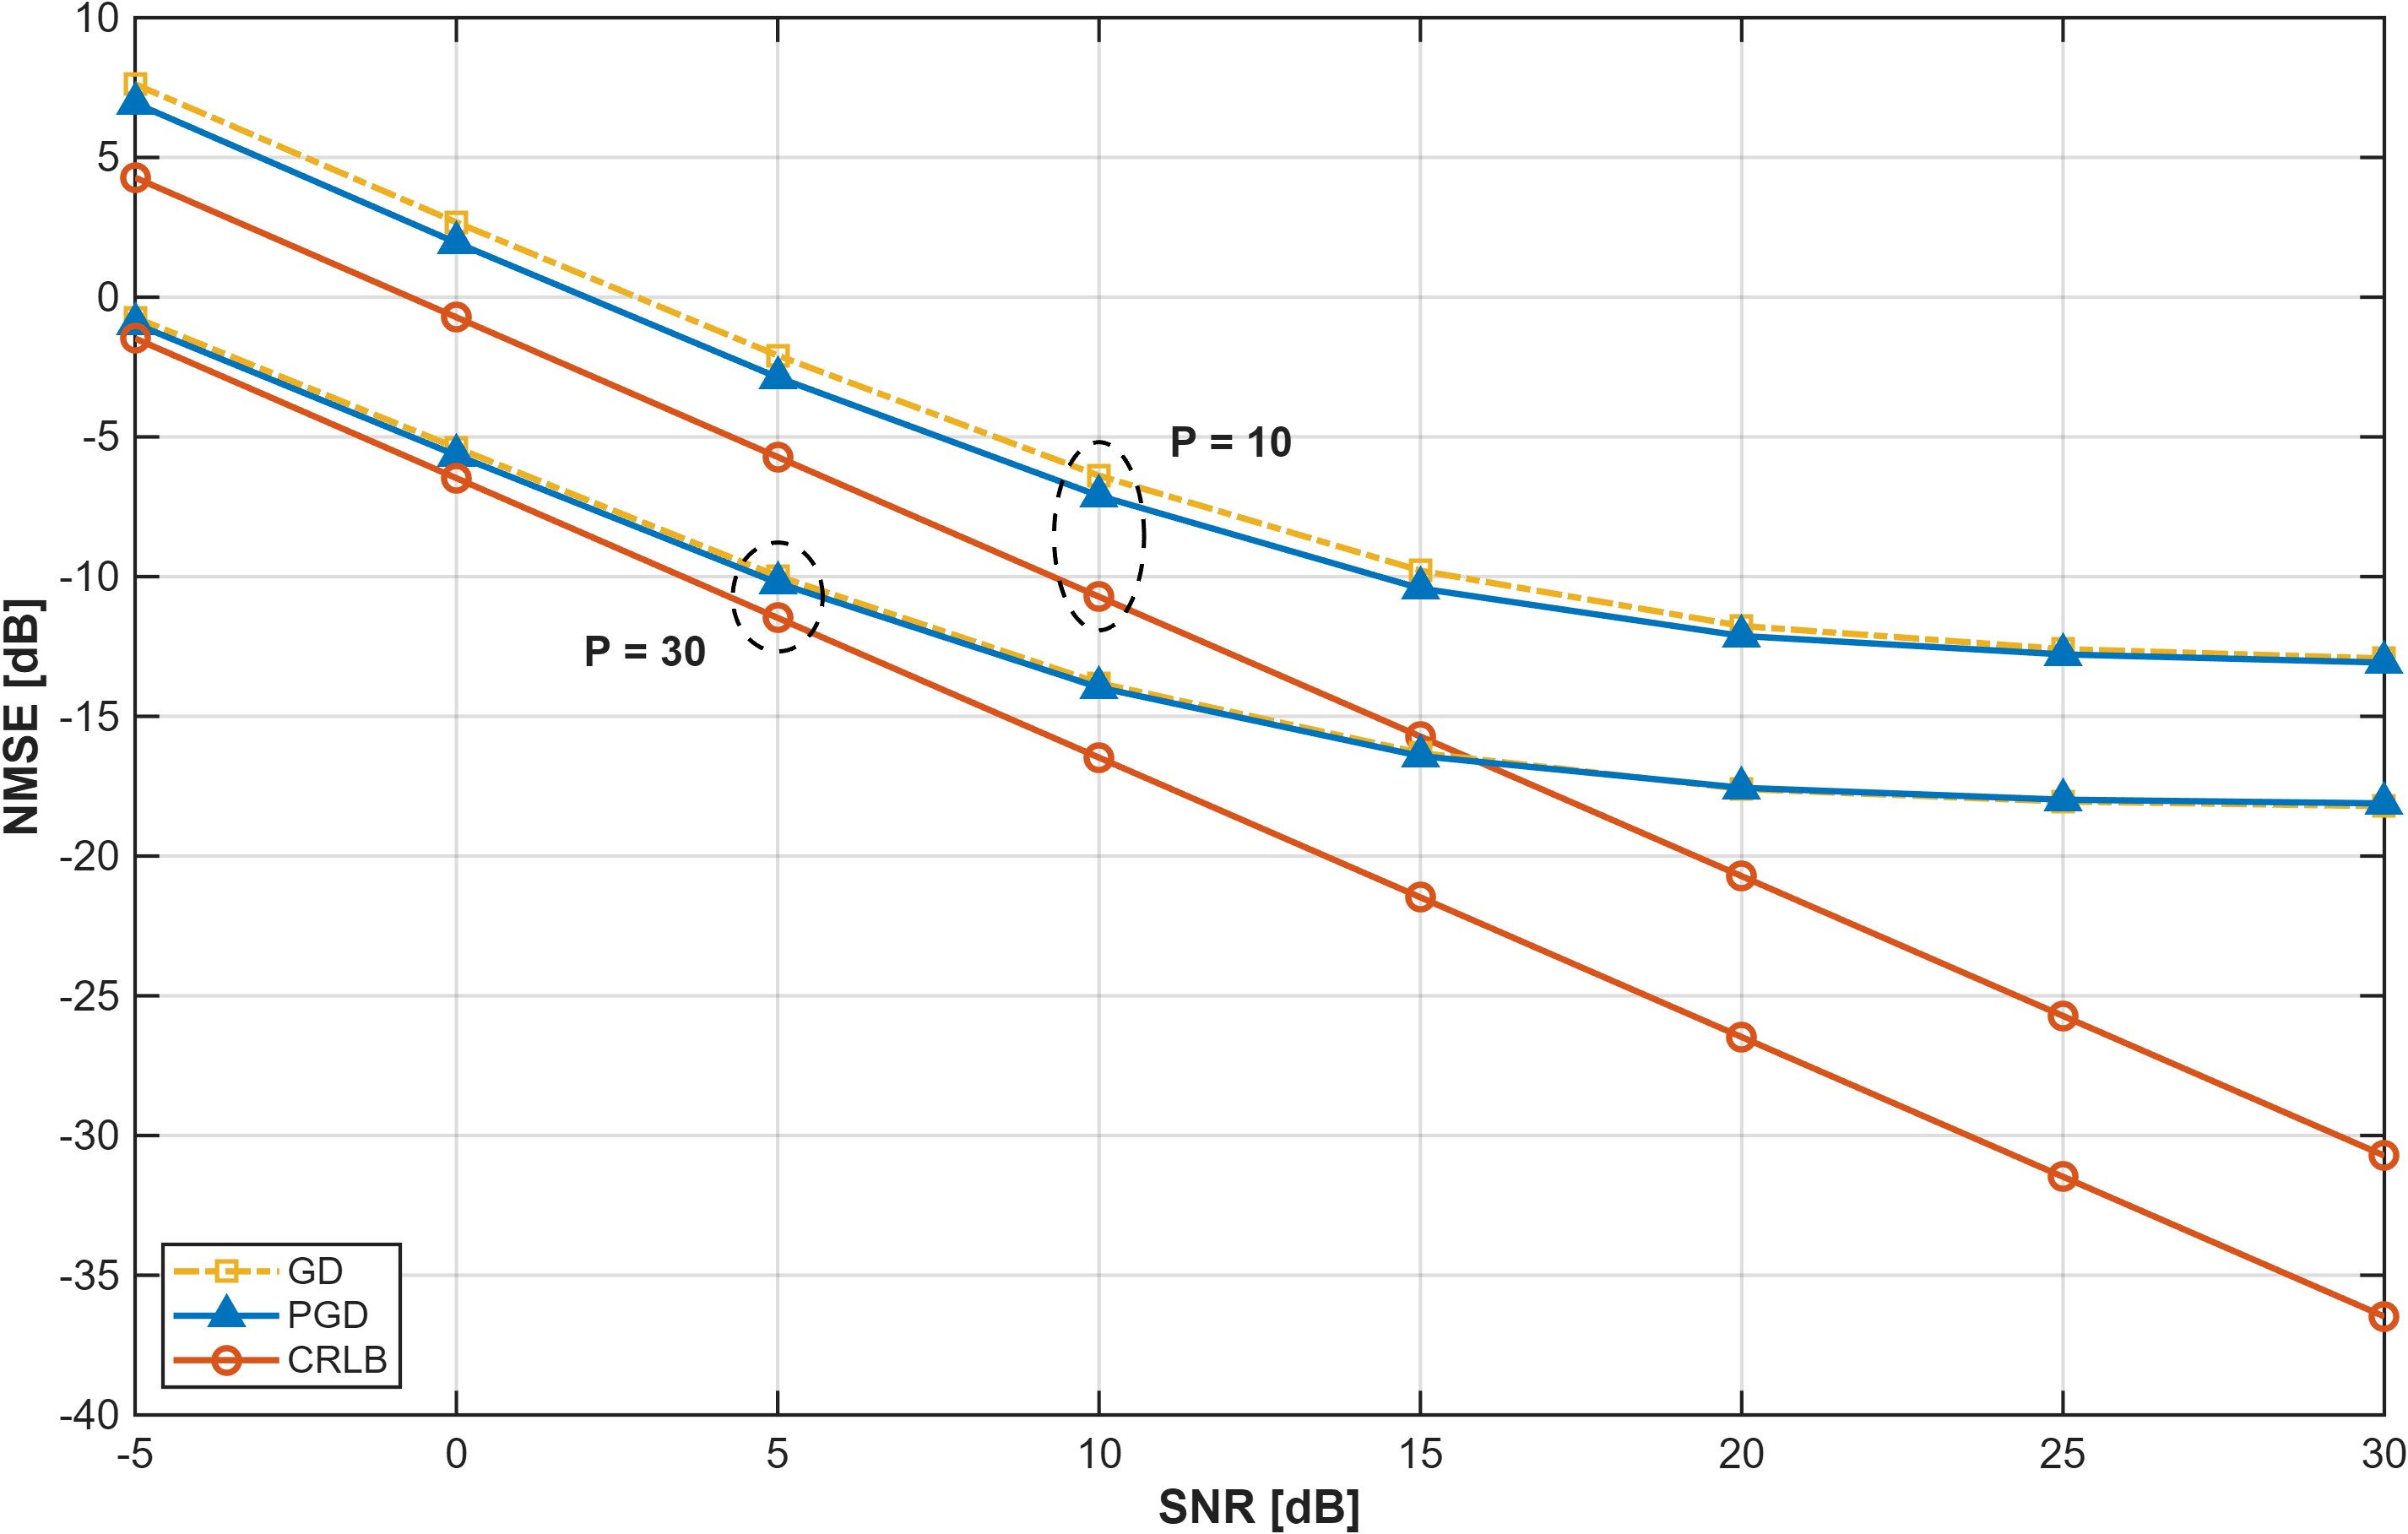
\includegraphics[width=\linewidth,height=0.52\textheight,keepaspectratio]{ce_fig4_2d.png}\\
  {\tiny NMSE vs SNR, $8\times8$ array: GD, PGD, CRLB}
\end{center}
\begin{itemize}\footnotesize\setlength\itemsep{1pt}
  \item $P=10$: PGD 0.6--0.8~dB better than GD (rank-$L_k$ projection)
  \item $P=30$: both within 1.3~dB of CRLB up to 5~dB SNR
\end{itemize}
\column{0.49\textwidth}
\begin{center}
  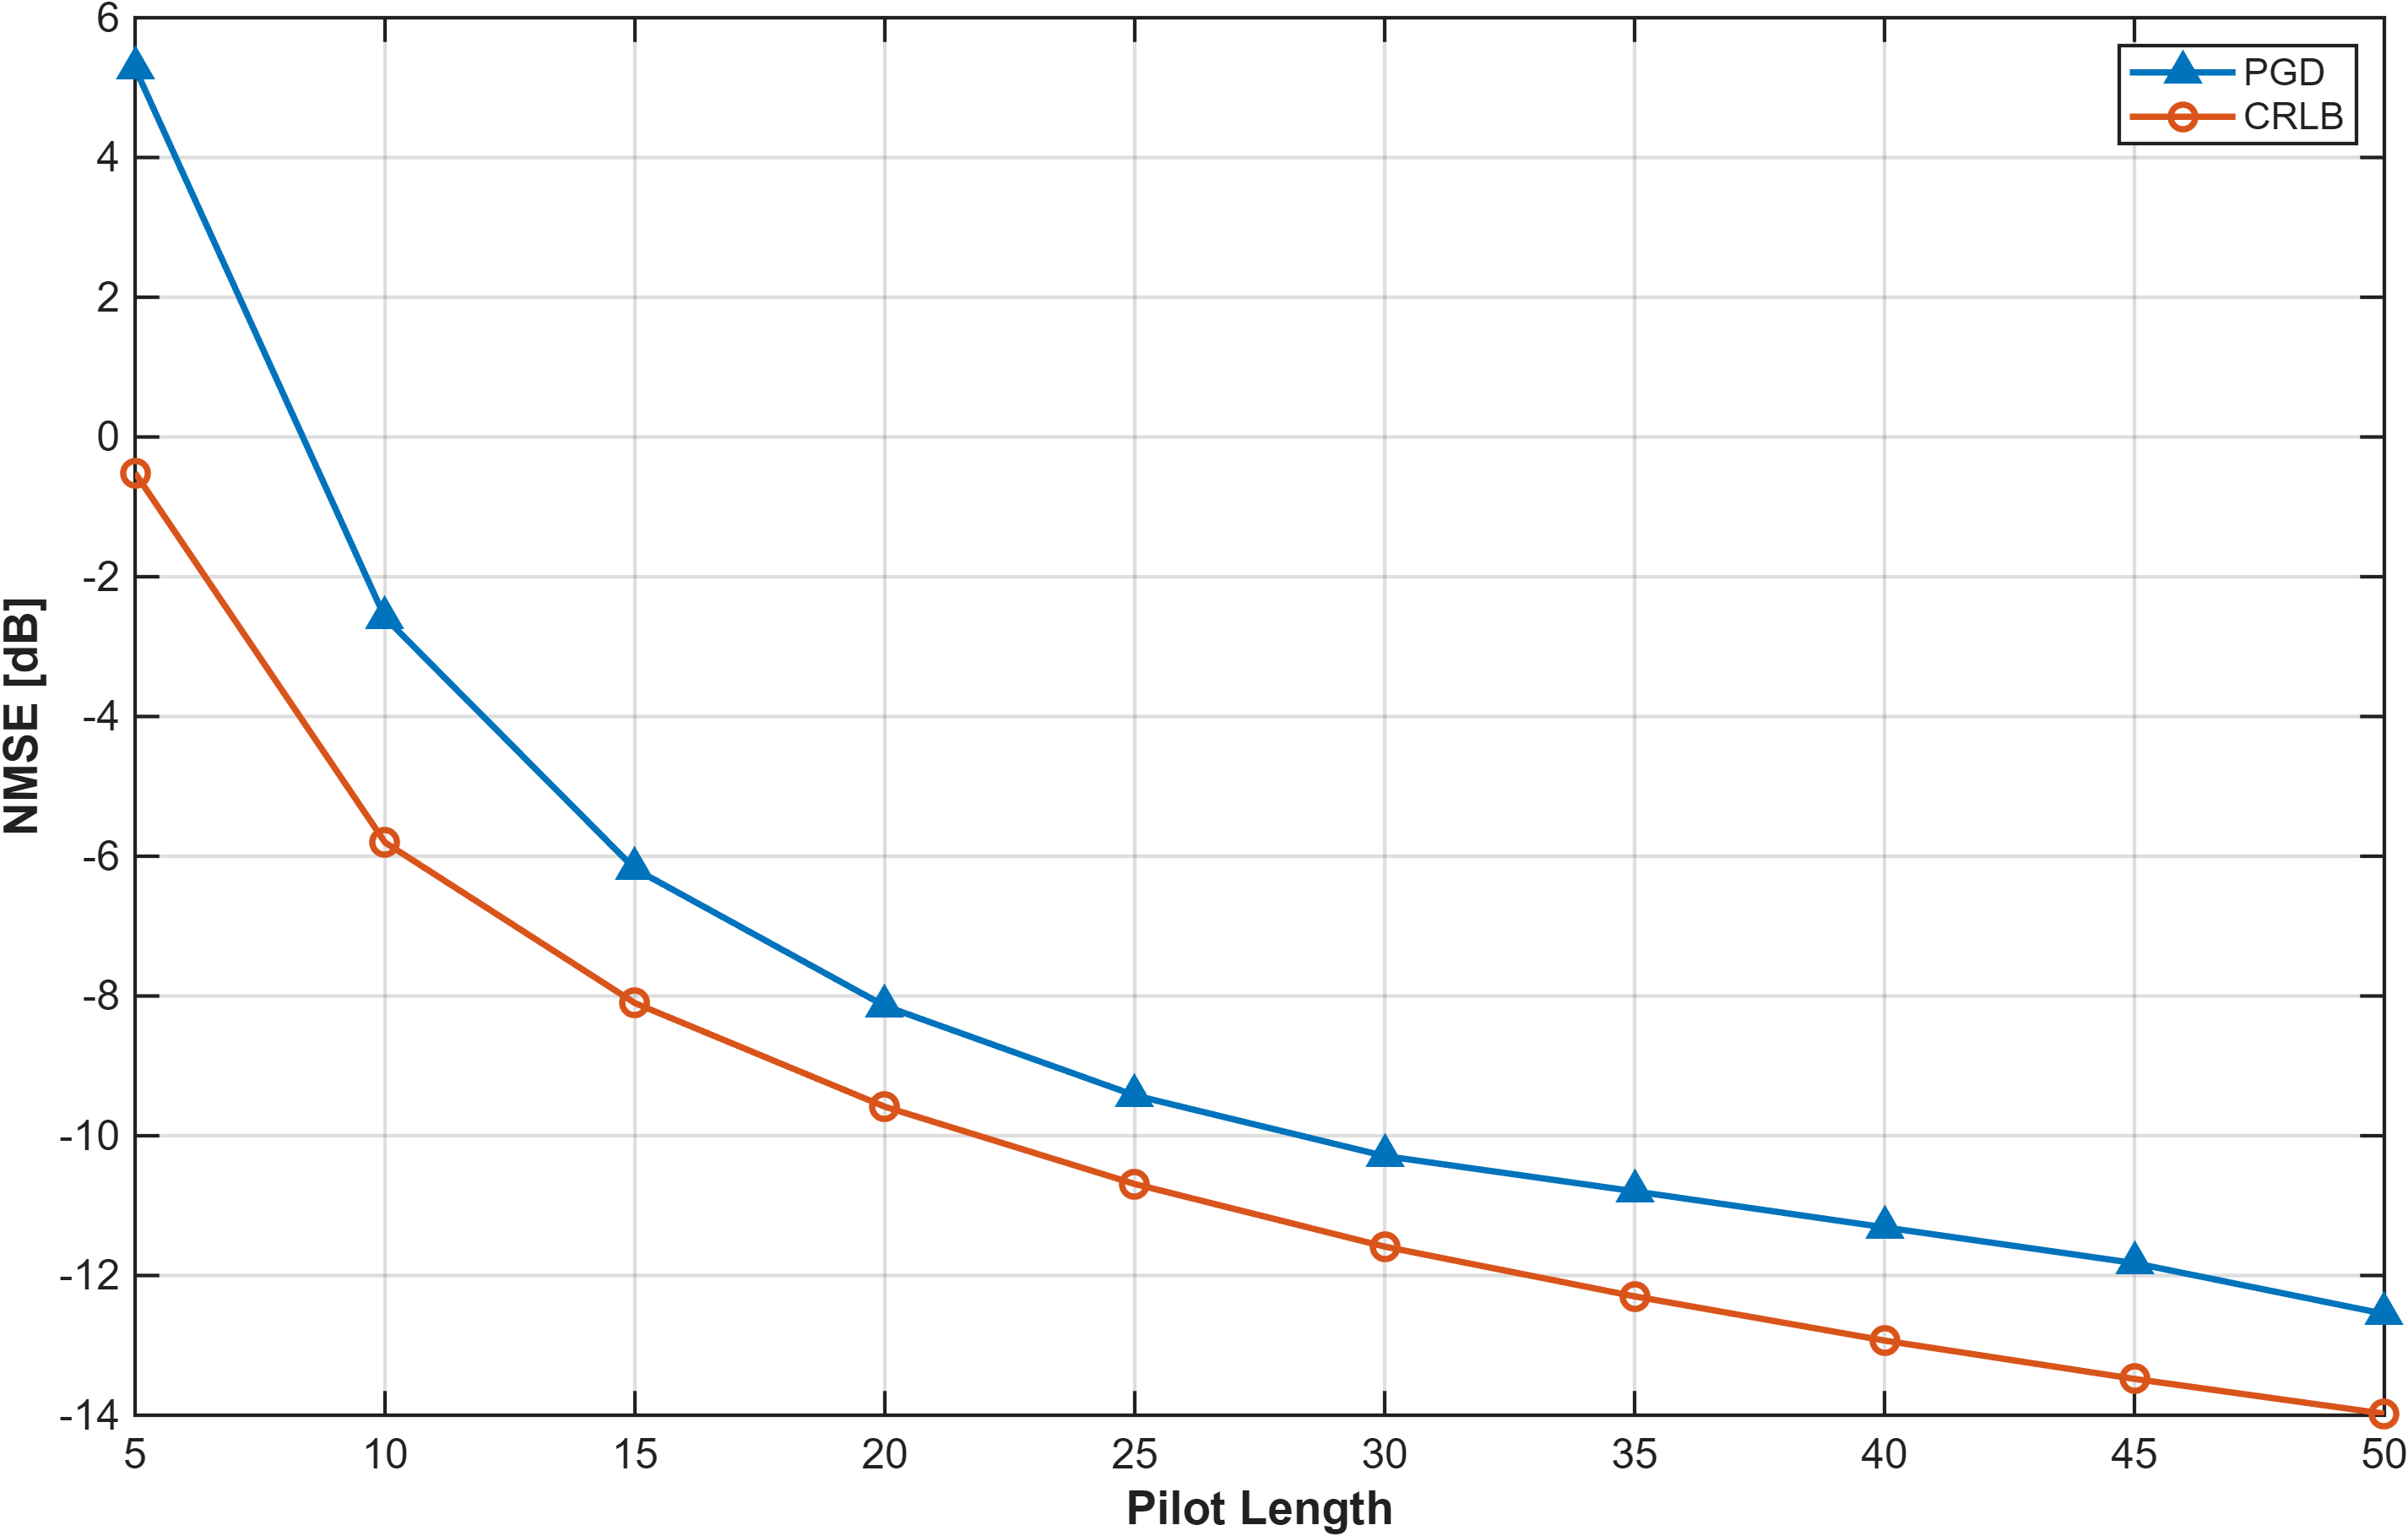
\includegraphics[width=\linewidth,height=0.52\textheight,keepaspectratio]{ce_fig5_pilot.png}\\
  {\tiny NMSE vs pilot length, $8\times8$ array, SNR = 5~dB}
\end{center}
\begin{itemize}\footnotesize\setlength\itemsep{1pt}
  \item Gap to CRLB: 5.8~dB ($P=5$) $\to$ 1.9~dB ($P=15$)
  \item 1.3--1.7~dB for $P\geq20$: about 20 pilots suffice
\end{itemize}
\end{columns}
\end{frame}

%% ---- 15. Gaps + future --------------------------------%% ---- 15. Gaps + future -----------------------------------
\begin{frame}{Research Gaps and Future Work}
\begin{enumerate}\small\setlength\itemsep{8pt}
    \item \textbf{Research gaps}
  \begin{itemize}\small\setlength\itemsep{3pt}
    \item Existing models assume only a strong reference; the weak-reference case is not considered
    \item Existing estimators (GD, GS, PGD) are iterative and need high computation time
    \item Learning-based channel estimation is not explored
    \item Effect of the estimated channels on data detection (SER/BER) is not evaluated
  \end{itemize}

  \item \textbf{Future work}
  \begin{itemize}\small\setlength\itemsep{3pt}
    \item Channel estimation based on CNN-based deep learning, Quantum machine learning (QML) and Hankel-structured methods, aiming for fewer iterations, lower computation time and high accuracy
    \item Compare these with the existing estimators (GD, GS, PGD) and the CRLB
    \item Data transmission using the CNN, QML and Hankel-structured channel estimates, and evaluation of SER and BER vs SNR

  \end{itemize}
\end{enumerate}
\end{frame}




%% ---- 16. References --------------------------------------
\begin{frame}{References}
\scriptsize
\begin{thebibliography}{9}
\setbeamertemplate{bibliography item}{\insertbiblabel}

\bibitem{cui2026rare}
M.~Cui, Q.~Zeng, and K.~Huang, ``Rydberg atomic receiver: Next frontier of wireless
communications,'' \textit{arXiv:2412.12485v1}, Dec. 2024.

\bibitem{chen2025harnessing}
Y.~Chen \textit{et al.}, ``Harnessing Rydberg atomic receivers: From quantum physics to
wireless communications,'' \textit{arXiv:2501.11842v1}, Jan. 2025.

\bibitem{cui2025towards}
M.~Cui, Q.~Zeng, and K.~Huang, ``Towards atomic MIMO receivers,'' \textit{IEEE J. Sel.
Areas Commun.}, vol.~43, no.~3, pp.~659--673, Mar. 2025.

\bibitem{xu2025channel}
B.~Xu \textit{et al.}, ``Channel estimation for Rydberg atomic receivers,''
\textit{IEEE Wireless Commun. Lett.}, vol.~14, no.~9, pp.~2957--2961, Sep. 2025.

\bibitem{liu2022deep}
Z.-K.~Liu, L.-H.~Zhang, B.~Liu, Z.-Y.~Zhang, G.-C.~Guo, D.-S.~Ding, and B.-S.~Shi, ``Deep
learning enhanced Rydberg multifrequency microwave recognition,'' \textit{Nature Commun.},
vol.~13, Art. no.~1997, Apr. 2022.

\bibitem{netrapalli2015}
P.~Netrapalli, P.~Jain, and S.~Sanghavi, ``Phase retrieval using alternating
minimization,'' \textit{IEEE Trans. Signal Process.}, vol.~63, no.~18, pp.~4814--4826,
Sep. 2015.

\bibitem{johansson2012qutip}
J.~R.~Johansson, P.~D.~Nation, and F.~Nori, ``QuTiP: An open-source Python framework for the
dynamics of open quantum systems,'' \textit{Comput. Phys. Commun.}, vol.~183, no.~8,
pp.~1760--1772, 2012.

\end{thebibliography}
\end{frame}

%% ---- Thank You -------------------------------------------
\begin{frame}[plain]
\begin{center}
  \vspace{1.5cm}
  {\Huge\textbf{Thank You}}\\[10pt]
  \rule{6cm}{0.5pt}
\end{center}
\end{frame}

\end{document}
